\documentclass[oneside,11pt]{amsart}
\usepackage[utf8]{inputenc}%
\usepackage[english]{babel}%
\usepackage{amsmath,amssymb,amsthm,amsfonts}%
\usepackage[unicode]{hyperref}%
\usepackage{mathrsfs,bbm}%
\usepackage{paralist}
\usepackage{color}
\usepackage{longtable}
\usepackage{array}
\newcolumntype{L}[1]{>{\small\raggedright\arraybackslash}m{#1}}
\newcolumntype{T}[1]{>{\footnotesize\raggedright\arraybackslash}m{#1}}
\usepackage{stmaryrd}%
%\usepackage{refcheck}
\usepackage{graphicx}
\usepackage[DIV17]{typearea}
\usepackage{multicol,tikz}
\usepackage{datetime}
\usepackage{cleveref}

\usepackage[shadow]{todonotes}

\usepackage{etoolbox}
\patchcmd{\section}{\scshape}{\Large\itshape\bfseries}{}{}

\usepackage{caption}
\captionsetup{labelformat=empty,labelsep=none}

\hypersetup{
  colorlinks=true,
  linkcolor=blue!50!red,
  urlcolor=green!60!black
}

%%%%%%%%%%%%%%%%%%%%%%%%%%%%%%%%%%%%%%%%%%%%%%%%%%%%%%%%%%%%%%%%%%%%%%%%%%%%%%%%%%%%%%%%
\synctex=1
%%%%%%%%%%%%%%%%%%%%%%%%%%%%%%%%%%%%%%%%%%%%%%%%%%%%%%%%%%%%%%%%%%%%%%%%%%%%%%%%%%%%%%%%
%%%%%%%%%%%%%%%%%%%%%%%%%%%%%%%%%%%%%%%%%%%%%%%%%%%%%%%%%%%%%%%%%%%%%%%%%%%%%%%%%%%%%%%%
\newcommand{\score}[1]{\textit{#1}\addtocounter{totalscore}{#1}}
\newcommand{\razdel}[1]{\smallskip\underline{\textbf{#1:}}\smallskip}

\newcommand{\note}[1]{{\sf{}\color{blue}(#1)}}

\begin{document}

\title[MATH 7310: REAL ANALYSIS AND LINEAR SPACES I]{MATH 7310: REAL ANALYSIS AND LINEAR SPACES I}
\author{Leonid Petrov\\Spring 2019}
\date{Compiled on \today, \currenttime.\\An up to date syllabus is always on \texttt{GitHub} at \url{https://github.com/lenis2000/Syllabi/blob/master/Syllabus_7310_s19.pdf}. For direct PDF download use \href{https://github.com/lenis2000/Syllabi/raw/master/Syllabus_7310_s19.pdf}{\texttt{this link}}.
	\LaTeX{} source with \textit{changes} to the syllabus is \href{https://github.com/lenis2000/Syllabi/blob/master/Syllabus_7310_s19.tex}{\texttt{here}}
(click ``History'').}
\maketitle

\bigskip

\section{Graduate real analysis}
\bigskip

This course introduces students to basic analytic tools used across all of mathematics:
\begin{itemize}
	\item Measures, including the Lebesgue measure on the line
	\item Lebesgue integration
	\item $L^p$ and Hilbert spaces
	\item Absolute continuity, differentiation of measures
\end{itemize}

Additional topics included in the course will range from applications to 
probability (e.g., theory of conditional expectations, Gaussian measures and Gaussian Free Field, \ldots)
to selected topics from classical analysis (orthogonal polynomials, numerical methods, steepest descent, \ldots),
as time permits.
Students' suggestions of additional topics are also welcome.

\begin{figure}[h]
	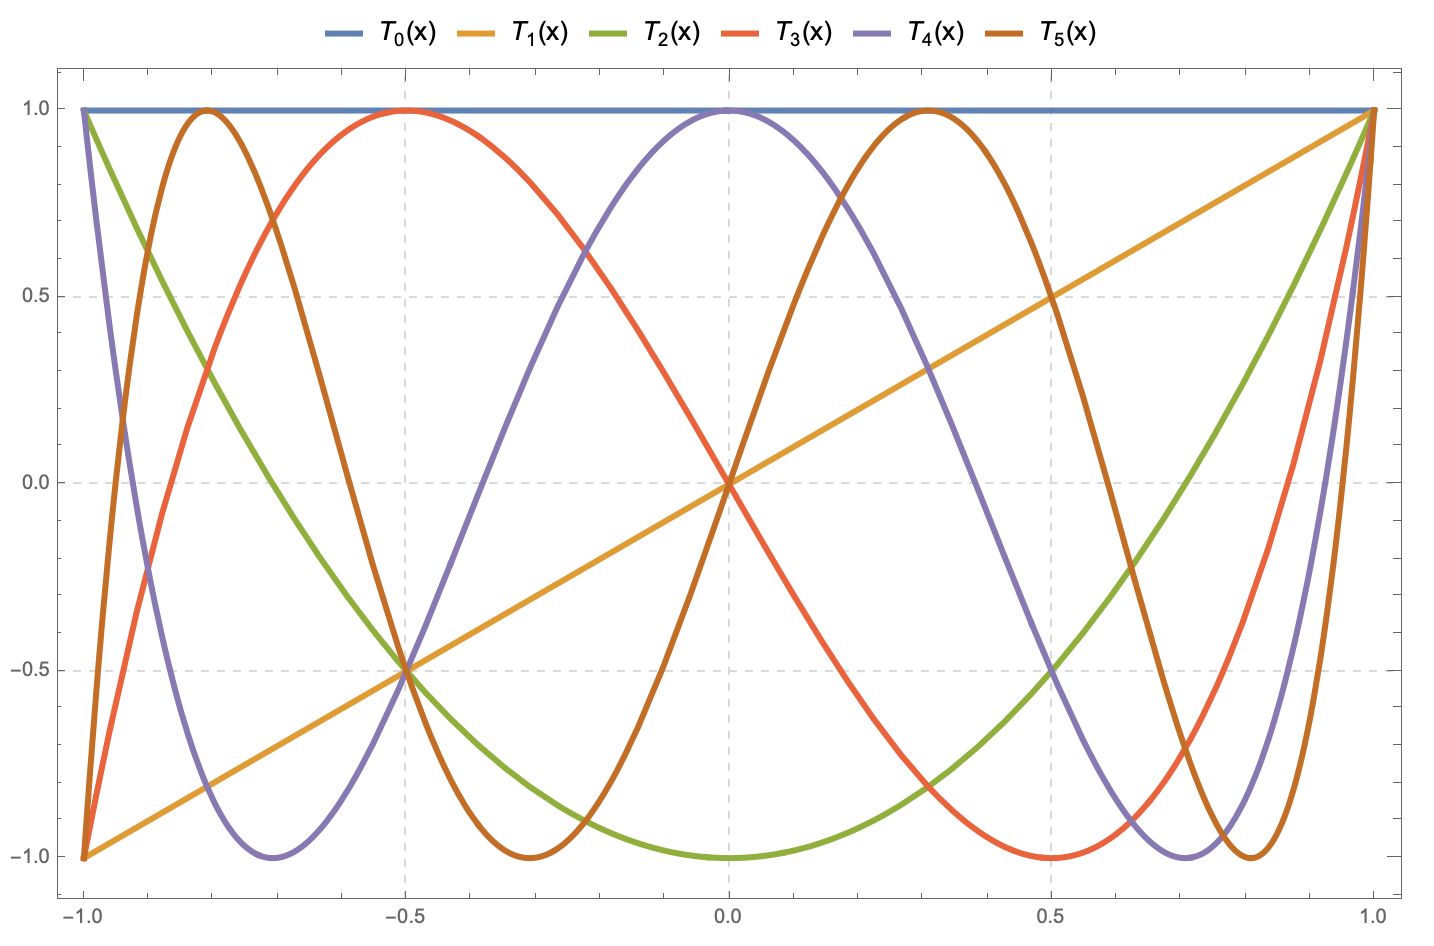
\includegraphics[height=.32\textwidth]{img/chebyshev.png}
	\caption{The first six Chebyshev polynomials of the first kind.}
\end{figure}

\subsection*{Prerequisites}

Single variable and multi-variable Calculus (limits and continuity,
differentiation and integration, series, uniform convergence, etc.), Linear
Algebra (vector spaces, linear mappings, matrices, determinants, etc.), and
some knowledge of set theory and topology of metric spaces. 


\section{Necessary information}
\bigskip

	\textbf{Class times:}   TuTh 2:00PM - 3:15PM in
	\emph{Kerchof Hall 317}

\medskip


\textbf{Exams:} Please do not make travel plans which conflict 
with the first midterm or the final exam.
\begin{itemize}
	\item \textbf{Midterm 1:} In-class on February 19 (class time).
	\item \textbf{Midterm 2:} Take home, due April 4.
	\item \textbf{Final exam:} Monday, May 6, 9-12.
\end{itemize}

\medskip

\textbf{Instructor:} Leonid Petrov
\medskip

\textbf{Email:} \email{petrov@virginia.edu} or \email{lenia.petrov@gmail.com}
\medskip

\textbf{Office:} 209 Kerchof Hall
\medskip

\textbf{Office hours:} 
Tuesday and Thursday 10-11am, except the weeks when I'm \href{https://lpetrov.cc/2018/05/travel-2019/}{\texttt{traveling}}.\footnote{Note:
this PDF has green clickable links.}
Also feel free to drop in with quick questions any time, or make 
appointments 
(you can make as many appointments as you want).

\medskip

\textbf{Course webpage:} 
This term we will be using Piazza for class discussion. The system is highly catered to getting you help fast and efficiently from classmates and myself. Rather than emailing questions, I encourage you to post your questions on Piazza. If you have any problems or feedback for the developers, email \email{team@piazza.com}.

Find our class page at \url{https://piazza.com/virginia/spring2019/math7310/home}

A collab page for homework submissions will also be set up.

\section{Books}

The exposition of each topic will follow one
of the following books:
\begin{itemize}
	\item \emph{Real analysis: modern techniques and applications}, by G.B. Folland
	\item \emph{Real and complex analysis}, by W. Rudin
	\item \emph{Real analysis: Measure Theory, Integration, and Hilbert Spaces},
		by E. Stein and R. Shakarchi
	\item \emph{Measure Theory and Fine Properties of Functions},
		by L. Evans and R. Gariepy
	\item \emph{An epsilon of room: pages from year three of a mathematical blog},
		by T. Tao
\end{itemize}
The first two books are considered ``main'', 
the other ones are optional but may be of use.
Lecture notes (in a hand-written format)
will be provided on Piazza. 

\section{Assessing your learning}

\section{Homework}


\subsection{Collaboration on homework assignments}
\label{collaboration}

Group work on homework problems is allowed and strongly encouraged.
Discussions are in general very
helpful and inspiring. Nevertheless, before talking to others, get well started
on the problems, and contribute your fair share to the process. 

When completing the written homework assignments, everyone must write up his or her own
solutions in their own words.
It is very important that you truly understand the homework solutions you hand
in, otherwise you may be unpleasantly surprised by your in-class test results.


\section{Policies}

\subsection{Laptops and smartphones}

Please do not use laptops and smartphones during the class.
You won't need them to participate in the discussions, but they may easily distract 
you or other students (or me!). If you absolutely must use a laptop, please sit in the back row.

\subsection{Late/make up work} Each assignment will have due date and time.
Late assignments are not accepted. There will also be no make ups for the midterm tests and the final exam.
However, if you have special needs, emergency, or unavoidable conflicts, please
let me know as soon as possible, so we can arrange a workaround.

\subsection{Honor Code} The University of Virginia Honor Code applies to this
class and is taken seriously. Collaboration on homework
assignments is allowed within the bounds discussed above 
in the corresponding section.
Any honor code violations will be referred to the
Honor Committee.

\subsection{Special needs}

All students with special needs requiring accommodations should present the
appropriate paperwork from the Student Disability Access Center (SDAC). It is
the student's responsibility to present this paperwork in a timely fashion and
follow up with the instructor about the accommodations being offered.
Accommodations for test-taking (e.g., extended time) should be arranged at
least 5 business days before an exam.






\end{document}
